\documentclass{article}
\usepackage{tikz, comment}
\usepackage{pifont}
\usepackage{fontspec, pgfplots}
\usetikzlibrary{arrows, decorations.markings, decorations.pathreplacing}
\begin{comment}
:Title: Not defined yet
:Tags: moment;focus of a parabola;polar coordinates;directrix of a parabola;latus rectum
:Prob: 0.4932;0.4768;0.4723;0.4684;0.4613
:Author: Prof.Hu Ji-shan, HKUST
:Slug: No name yet

Description Here.........
\end{comment}
\begin{document}\centering 

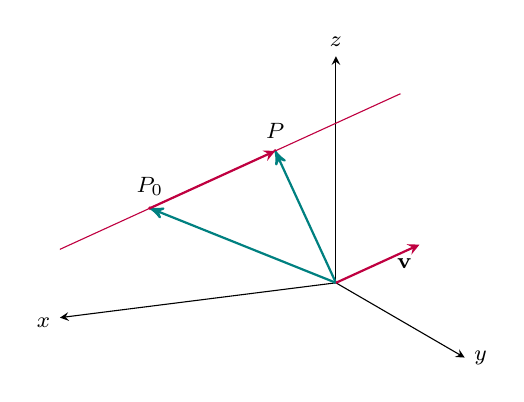
\begin{tikzpicture}[font=\footnotesize]
\pgfplotsset{compat=1.8}
\begin{axis}
[axis lines = center, view={155}{20}, ticks=none, scale=0.75,
axis background, xlabel = {$x$}, ylabel ={$y$}, zlabel ={$z$}, domain =-2:2, y domain =-2:2,
xmin =0,
xmax =3.99,
ymin =0,
ymax =2.99,
zmin =0, 
zmax =4,
samples =10, samples y =40, z buffer = auto, 
every axis x label/.style={
    at={(ticklabel* cs:1)},
    anchor= east, yshift =-2
},
every axis y label/.style={
    at={(ticklabel* cs:1)},
    anchor= west,
},
every axis z label/.style={
    at={(ticklabel* cs:1)},
    anchor= south
}]

\addplot3 [data cs=cart, purple, domain=0:1, y domain = -1:2.3] ({3+y*(-3)},{0.5+y*1},{2+y*2});

\node[label={90:{$P_0$}}, purple, circle,fill,inner sep=0.5pt] at (axis cs:3,0.5,2) {};
\node[label={90:{$P$}}, purple, circle,fill,inner sep=0.5pt] at (axis cs:1.5,1,3) {};
\node[label={0:{${\bf v}$}}] at (axis cs:-0.5,0.166667,0.333333) {};

\addplot3 [teal, thick, ->, >=stealth'] coordinates
{ (0,0,0) (3,0.5,2) };

\addplot3 [teal, thick, ->, >=stealth'] coordinates
{ (0,0,0) ({3+0.5*(-3)},{0.5+ 0.5*1},{2+ 0.5*2}) };

\addplot3[purple, thick, ->, >=stealth] coordinates
{ (3,0.5,2) (1.5,1,3) };

\addplot3[purple, thick, ->, >=stealth] coordinates
{ (0, 0, 0) ({-0.5*2},{0.166667*2},{0.333333*2}) };

\end{axis}

\end{tikzpicture}
\end{document}